% $Header: /cvsroot/latex-beamer/latex-beamer/solutions/conference-talks/conference-ornate-20min.en.tex,v 1.6 2004/10/07 20:53:08 tantau Exp $

\documentclass[usenames,dvipsnames]{beamer}

\mode<presentation>
{
%  \usetheme{Hannover}
\usetheme[width=0.7in]{Hannover}
% or ...

  \setbeamercovered{transparent}
  % or whatever (possibly just delete it)
}
\usepackage{longtable}
\usepackage{booktabs}
\usepackage{bnf}
\usepackage{bm}

%\usepackage{qtree}

\usepackage[english]{babel}
% or whatever

\usepackage[latin1]{inputenc}
% or whatever

\usepackage{times}
%\usepackage[T1]{fontenc}
% Or whatever. Note that the encoding and the font should match. If T1
% does not look nice, try deleting the line with the fontenc.
%\usepackage{logictheme}

\usepackage{multirow}
\usepackage{totpages}
\usepackage{hyperref}
\usepackage{booktabs}
\usepackage[round]{natbib}

\usepackage{listings}
% \lstset{frame=none, showstringspaces=false, basicstyle=\ttfamily\footnotesize,
%   xleftmargin=-8mm,language=Haskell}
\lstset{frame=none, showstringspaces=false, basicstyle=\ttfamily\bfseries\footnotesize,
  xleftmargin=-8mm,language=Haskell,breaklines=true}

\usepackage{tikz}
\usetikzlibrary{positioning}

\hypersetup{colorlinks=true,
    linkcolor=blue,
    citecolor=blue,
    filecolor=blue,
    urlcolor=blue,
    unicode=false}

\usepackage{pifont}
\usepackage{amsmath, amsfonts, amssymb, xspace, xcolor, url}
\newcommand{\cross}{{\LARGE {\color{red}\ding{55}}}}

\newcommand{\greencheck}{{\LARGE {\color{ForestGreen}\checkmark}}}
\newcommand{\bluedash}{{\LARGE {\color{blue}{--}}}}

\newcommand{\blt}{- } %used for bullets in a list

\newcounter{datadefnum} %Datadefinition Number
\newcommand{\ddthedatadefnum}{DD\thedatadefnum}
\newcommand{\ddref}[1]{DD\ref{#1}}

\newcommand{\colAwidth}{0.1\textwidth}
\newcommand{\colBwidth}{0.8\textwidth}

\renewcommand{\arraystretch}{1.1} %so that tables with equations do not look crowded

\pgfdeclareimage[height=0.7cm]{logo}{McMasterLogo}
\title[\pgfuseimage{logo}] % (optional, use only with long paper titles)
{A Holistic Approach to Pain Relief for Research Software Developers}

%\subtitle
%{Include Only If Paper Has a Subtitle}

\author[Slide \thepage~of \pageref{TotPages}] % (optional, use only with lots of
                                              % authors)
{\textbf{Spencer Smith}, Jacques Carette}
% - Give the names in the same order as the appear in the paper.
% - Use the \inst{?} command only if the authors have different
%   affiliation.

\institute[McMaster University] % (optional, but mostly needed)
{
  Computing and Software Department\\
  Faculty of Engineering\\
  McMaster University
}
% - Use the \inst command only if there are several affiliations.
% - Keep it simple, no one is interested in your street address.

\date[May 31, 2022] % (optional, should be abbreviation of conference name)
{Canadian Research Software Conference, Montr\'eal, May 31--June 1, 2022}
% - Either use conference name or its abbreviation.
% - Not really informative to the audience, more for people (including
%   yourself) who are reading the slides online

\subject{research software, software engineering, literate programming, code
  generation}
% This is only inserted into the PDF information catalog. Can be left
% out. 

% If you have a file called "university-logo-filename.xxx", where xxx
% is a graphic format that can be processed by latex or pdflatex,
% resp., then you can add a logo as follows:

%\pgfdeclareimage[height=0.5cm]{Mac-logo}{McMasterLogo}
%\logo{\pgfuseimage{Mac-logo}}

% Delete this, if you do not want the table of contents to pop up at
% the beginning of each subsection:
% \AtBeginSubsection[]
% {
%   \begin{frame}<beamer>
%     \frametitle{Outline}
%     \tableofcontents[currentsection,currentsubsection]
%   \end{frame}
% }

% If you wish to uncover everything in a step-wise fashion, uncomment
% the following command: 

%\beamerdefaultoverlayspecification{<+->}

\beamertemplatenavigationsymbolsempty 

% have SRS and LP open during the presentation

\begin{document}

%%%%%%%%%%%%%%%%%%%%%%%%%%%%%%%%%%%%%%
\hoffset=-.4in %removing side bar for these frames
\begin{frame}[plain]

\begin{tikzpicture}[remember picture,overlay]
  \node [xshift=1.3cm,yshift=0cm] at (current page.center)
  {
  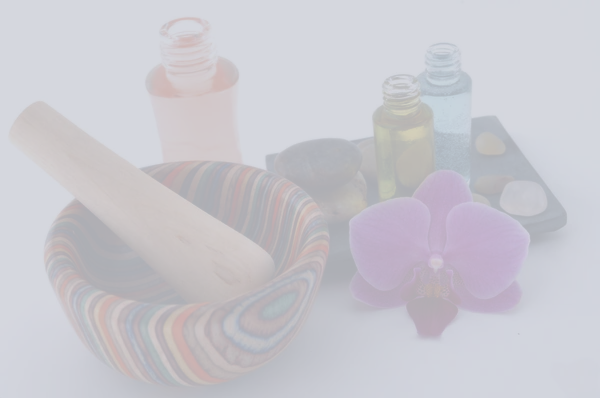
\includegraphics[width=1.5\textwidth]{holisticFaint.png}
  };
\end{tikzpicture}

\titlepage

\end{frame}
\hoffset=0in %restore
%%%%%%%%%%%%%%%%%%%%%%%%%%%%%%%%%%%%%%

% \begin{frame}

% \frametitle{Literate Scientific Software}
% \tableofcontents
% % You might wish to add the option [pausesections]

% % make like a story - the phases - reason for, why works, advantages
% % changing the history a bit to make a more rational narrative

% \end{frame}

%%%%%%%%%%%%%%%%%%%%%%%%%%%%%%%%%%%%%%

\begin{frame}

\frametitle{Outline}

\begin{itemize}
  \item Sustainable and Reproducible Research Software %Health Goal
  \item Pain Points
  \item Treatment Options
  \begin{itemize}
    \item Literate Programming %other options out of scope
    \item Code Generation
    \item Holistic Approach
  \end{itemize}
  \item Concluding Remarks
\end{itemize}

\begin{tikzpicture}[remember picture,overlay]
  \node [xshift=3.4cm,yshift=-2.0cm] at (current page.center)
  {
  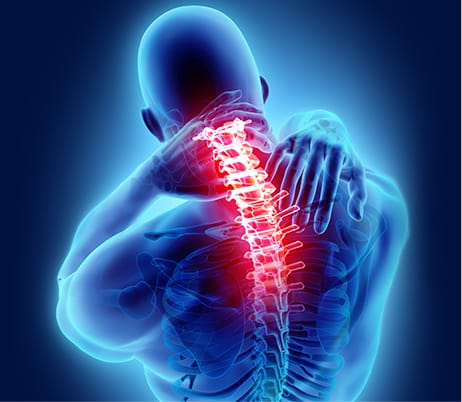
\includegraphics[width=0.47\textwidth]{backpain.jpeg}
  };
\end{tikzpicture}
  
\end{frame}

%%%%%%%%%%%%%%%%%%%%%%%%%%%%%%%%%%%%%%

\section[Health Goals]{Health Goals and Pain Points}

%%%%%%%%%%%%%%%%%%%%%%%%%%%%%%%%%%%%%%

\begin{frame}

\frametitle{Health Goals}

\begin{itemize}
    % \item ``Sustainable development is development that meets the needs of the
    % present without compromising the ability of future generations to meet their
    % own needs.'' \citep{Brundtland1987}
    \item \textbf{Sustainable} software satisfies, for a reasonable amount of
    effort, the software \emph{requirements} for the present (like
    \emph{correctness}), while also being maintainable, reusable, and
    \emph{reproducible} for the future.
    \item \textbf{Reproducible} research includes all data, code, and
    documentation so that the computations can be \emph{repeated in the future
    with identical results}.
\end{itemize}

~\\
Requires design, documentation, and verification (testing)

\end{frame}

%%%%%%%%%%%%%%%%%%%%%%%%%%%%%%%%%%%%%%

\begin{frame}

\frametitle{Problems with Achieving Goals: Pain Points}

\vspace{-1.5cm}
% not trying to cover all pain points, just focusing on these, there are others
From Developer Interviews:
\begin{itemize}
\item Lack of time
\item Lack of software development experience %(especially for design)
\item Lack of technology experience %(tool support can help, but need time)
\item Frequency of change
\end{itemize}

\begin{tikzpicture}[remember picture,overlay]
  \node [xshift=3.2cm,yshift=-2.5cm] at (current page.center)
  {
  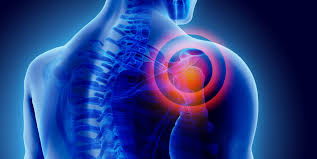
\includegraphics[width=0.47\textwidth]{shoulder.jpeg}
  };
\end{tikzpicture}

\end{frame}

%%%%%%%%%%%%%%%%%%%%%%%%%%%%%%%%%%%%%%

\section[Literate]{Literate Programming}

%%%%%%%%%%%%%%%%%%%%%%%%%%%%%%%%%%%%%%

\begin{frame}

  \frametitle{Treatment 1: Literate Programming}

  \begin{itemize}
  \item ``instead of imagining that our main task is to instruct a computer what
  to do, let us concentrate rather on explaining to human beings what we want a
  computer to do'' \citep[pg. 99]{Knuth1984}
  \item Interconnected ``web'' of pieces of code, or \emph{chunks}
  %\item Documentation with code, opposed to code with documentation %like doxygen etc.
  \item Tangle extracts code
  \item Weave extracts docs (as LaTeX, html, pdf, text, etc.)
  \item CWEB, Sweave (R), Jupyter, emacs org mode, Maple worksheets, etc.
  \end{itemize}

  \begin{tikzpicture}[remember picture,overlay]
    \node [xshift=3.4cm,yshift=-3.7cm] at (current page.center)
    {
    
\includegraphics[width=0.4\textwidth]{openbook.jpeg}
    };
  \end{tikzpicture}
  
\end{frame}
  
%%%%%%%%%%%%%%%%%%%%%%%%%%%%%%%%%%%%%%

\begin{frame}

  %\frametitle{Fuel Pellet Representation}
  
  \begin{center}
   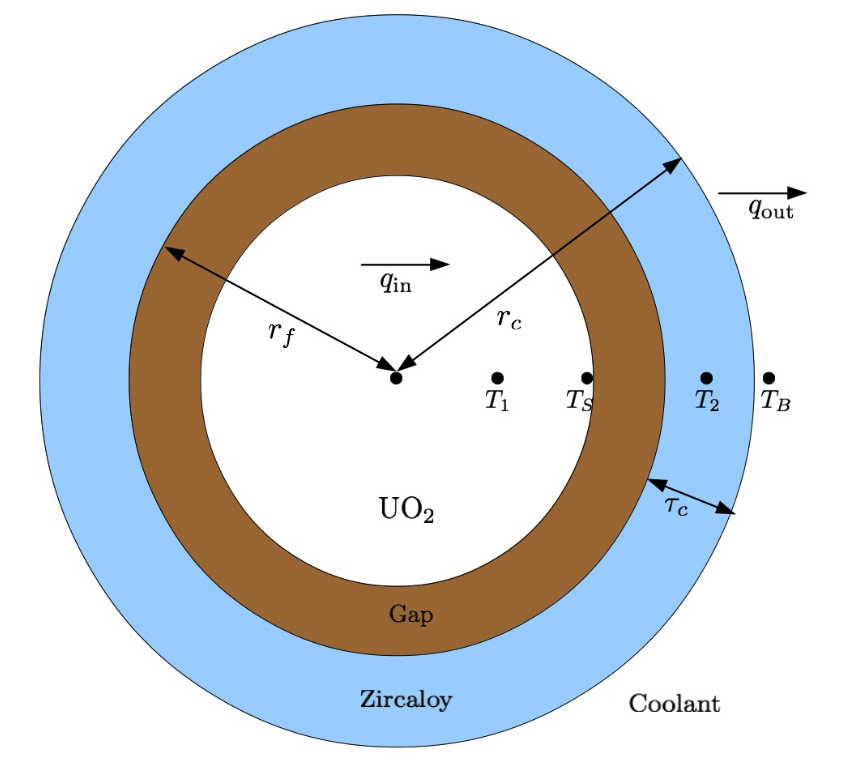
\includegraphics[width=0.6\columnwidth]{fuelpin.png}
  \end{center}
  
  \begin{center}
  %\rotatebox{-90}
  {
   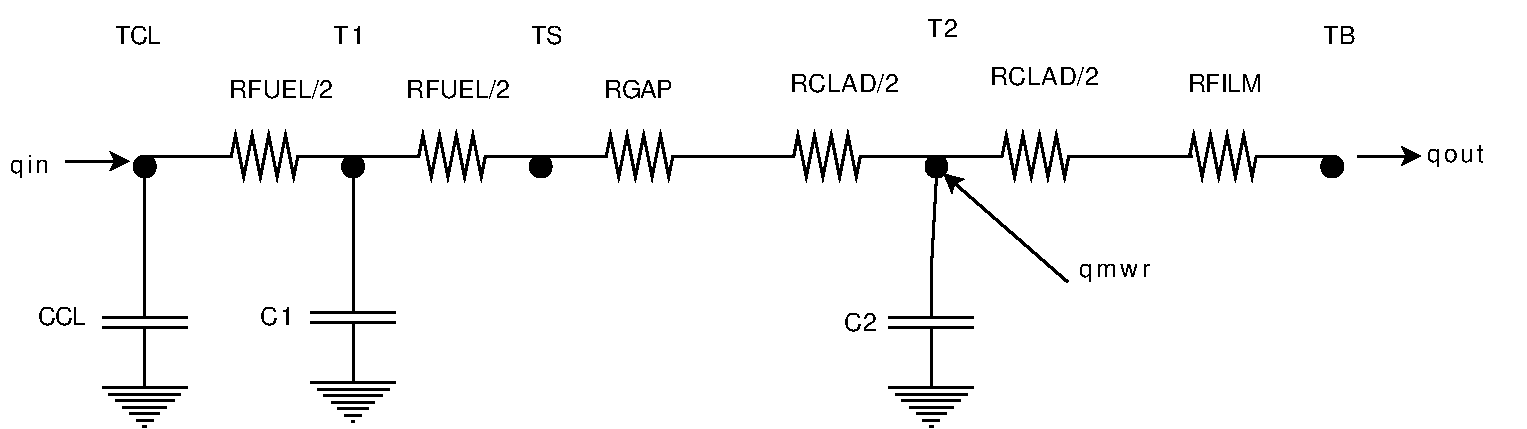
\includegraphics[width=1.0\columnwidth]{electricalcircuitanalogue.pdf}
  }
  \end{center}
  
\end{frame}
  
%%%%%%%%%%%%%%%%%%%%%%%%%%%%%%%%%%%%%%
\hoffset=-.4in %removing side bar for these frames
\begin{frame}[plain]
  
  \frametitle{Example}
  
  \hspace{-1.1cm}
  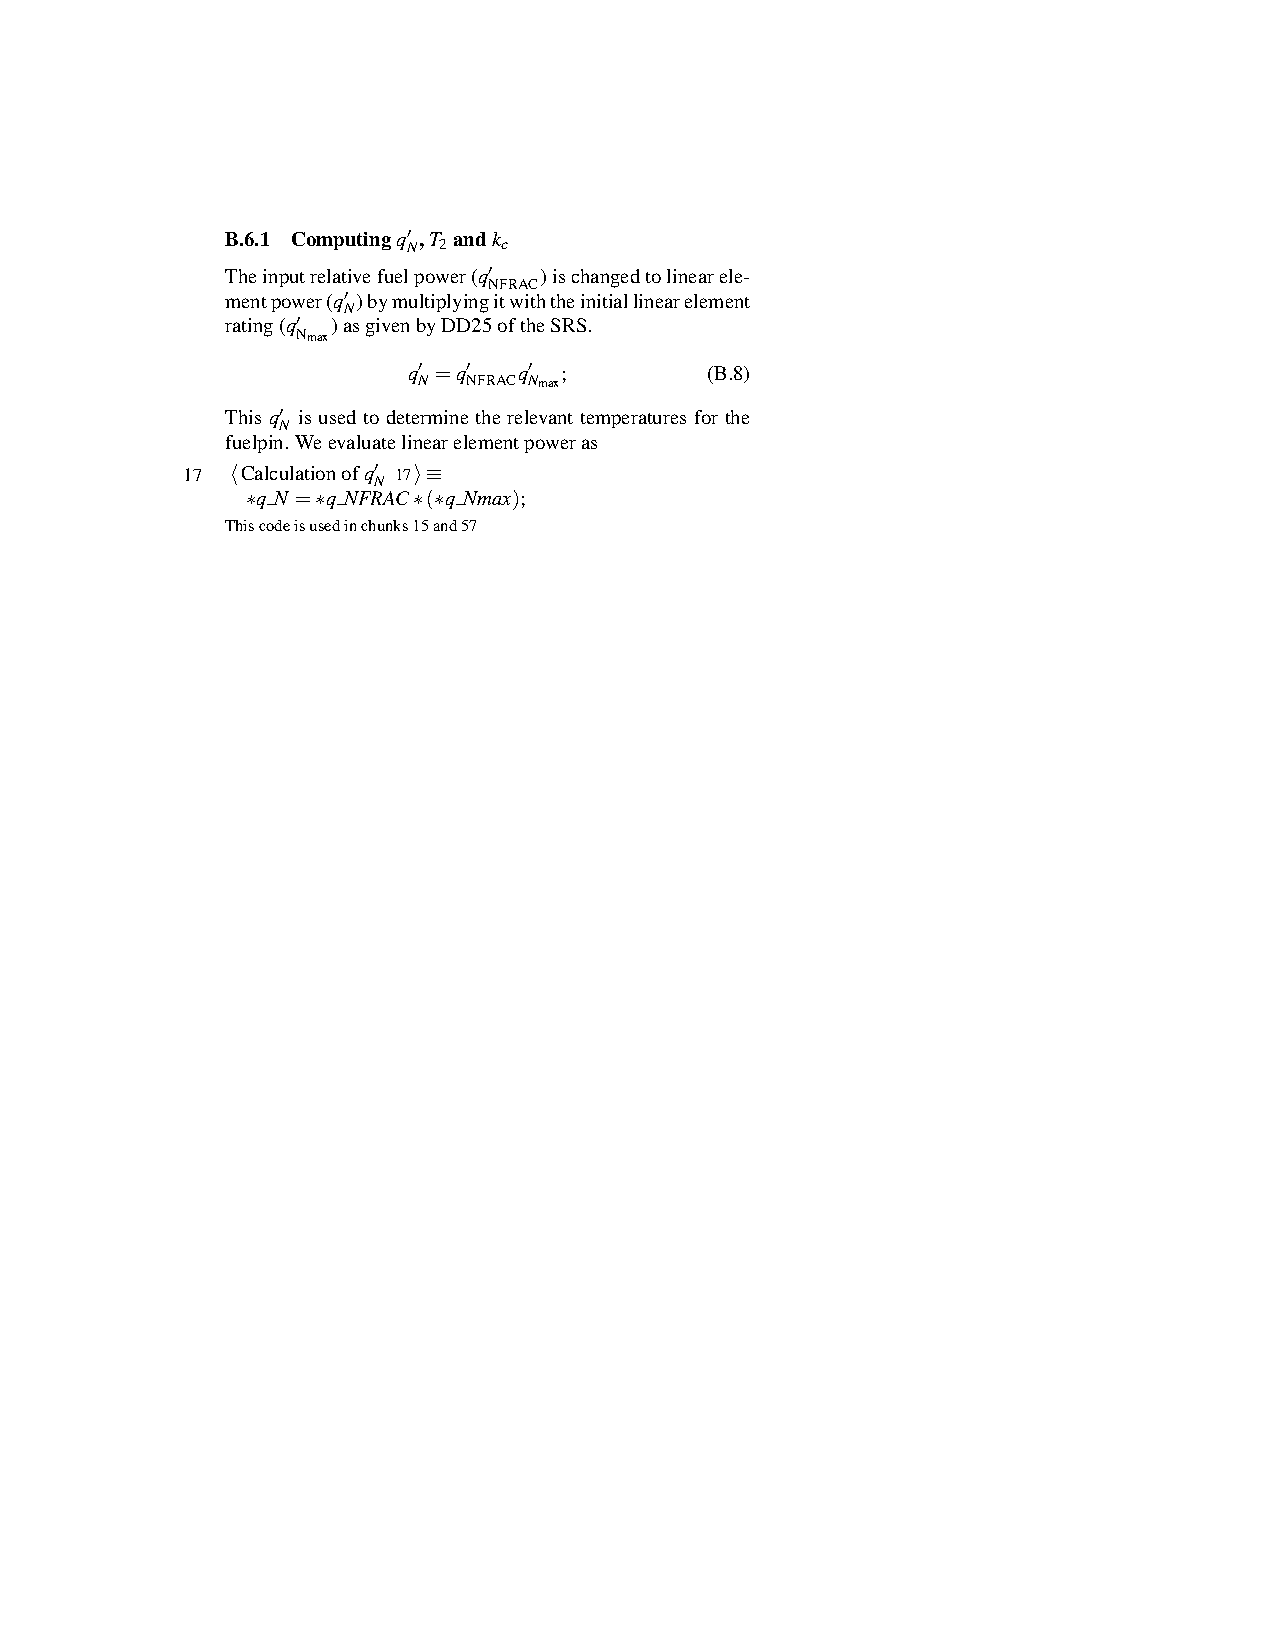
\includegraphics[width=1.1\columnwidth]{qnfrac.pdf}
  
\end{frame}
\hoffset=0in %restore
%%%%%%%%%%%%%%%%%%%%%%%%%%%%%%%%%%%%%%
  
\begin{frame}
  
  \frametitle{LP Treatment Evaluation}
  
  \begin{itemize}
  \item Uncovered 27 issues with previous docs
  \item Documentation improves reproducibility
  \item Pain point score:
  \begin{itemize}
    \item Lack of time: \greencheck %-- forces developers to find time for documentation
    \item Lack of dev exp: \bluedash %NEUTRAL %-- offers no design advice
    \item Lack of technology exp: \cross %-- exacerbates this problem
    \item Freq of change: \greencheck % -- code and documentation are maintained together
  \end{itemize}
  \item Problems with literate programming
  \begin{itemize}
    \item Does not scale well (best for small examples, lessons) %user guides
    \item Difficult to refactor
    \item \emph{Manually} repeat information in text and code
    \item \emph{Manually} create traceability and structure
    %\item Requirements usually left out
  \end{itemize}
  \end{itemize}

\end{frame}
  
%%%%%%%%%%%%%%%%%%%%%%%%%%%%%%%%%%%%%%

\section[Code Gen]{Code Generation}

%%%%%%%%%%%%%%%%%%%%%%%%%%%%%%%%%%%%%%

\begin{frame}

  \frametitle{Treatment 2: Code Generation}
  
  \hspace{2cm}

  %Code that writes code

  \begin{tikzpicture}[remember picture,overlay]
    \node [xshift=0.7cm,yshift=0.cm] at (current page.center)
    {
    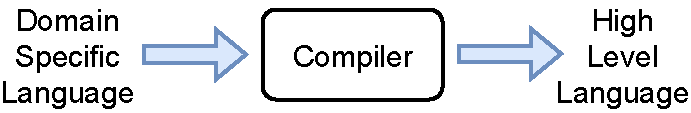
\includegraphics[width=1\textwidth]{compiler.pdf}
    };
  \end{tikzpicture}
  
\end{frame}
  
%%%%%%%%%%%%%%%%%%%%%%%%%%%%%%%%%%%%%%
  
\begin{frame}
  
  \frametitle{A Virtual Material Testing Laboratory}
  
  Given the deformation history of a material particle, determine the internal
  stress within the material particle.
  
  \begin{center}
  {
  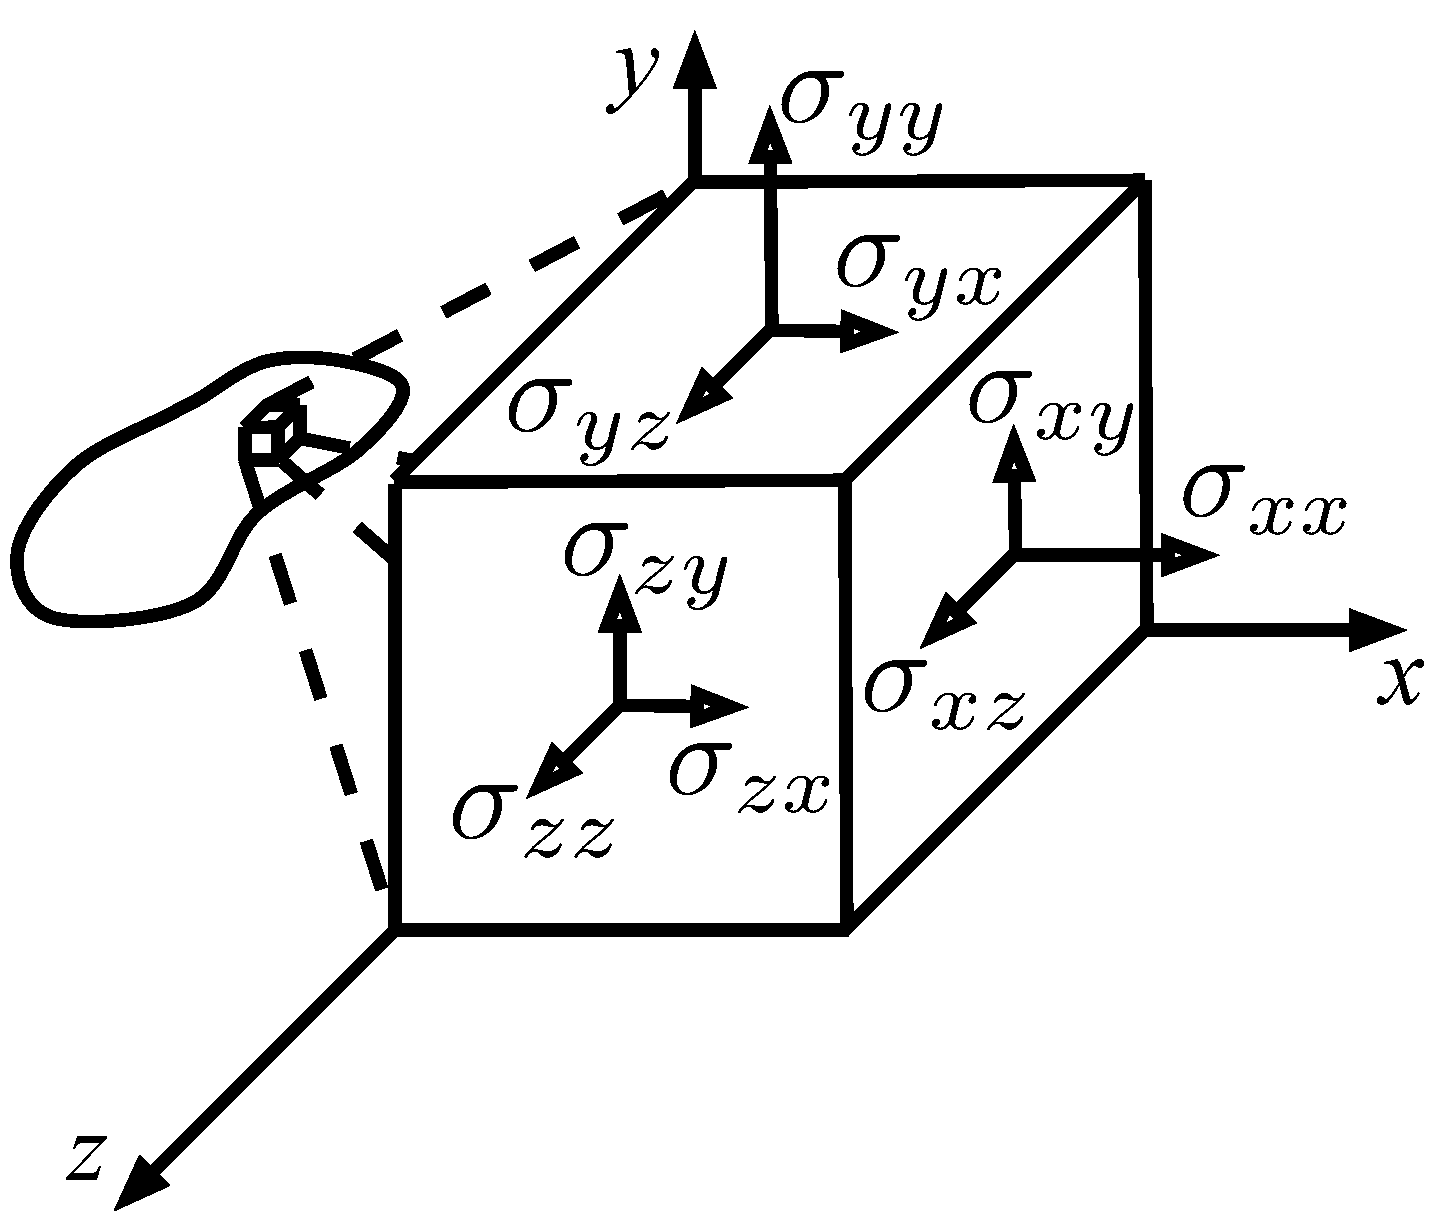
\includegraphics[width=0.65\textwidth]{StressTensor.pdf}
  }
  \end{center}
  
  \end{frame}
  
%%%%%%%%%%%%%%%%%%%%%%%%%%%%%%%%%%%%%%%%%%%%%%%%%%%%%%%%%%%%%%
  
\begin{frame}
  
  \frametitle{Calculations}
  
  Given $F, Q, \kappa, \phi, \gamma$ calculate:

  \begin{equation} \label{EqImplicitFEM}
    \mathbf{K} = \int_V \mathbf{B}^T \mathbf{D}^{vp} \mathbf{B} dV; \mathbf{F} = \mathbf{R}_i - \int_V \mathbf{B}^T \bm{\sigma}_i dV + \int_V \mathbf{B}^T
    \Delta
    \bm{\sigma}^{vp} dV
    \end{equation}
    with
    \begin{equation}
    \mathbf{D}_{vp} =
    \mathbf{D} \left [
    \mathbf{I} - {\Delta t} C_1 \lambda' \frac{\partial Q}{\partial \bm{\sigma}} \left ( \frac{\partial F}{\partial
    \bm{\sigma}} \right )^{T} \mathbf{D}
    \right ], \lambda' = \frac{d \lambda}{d F}
    \end{equation}
    \begin{equation}
    \Delta \bm{\sigma}^{vp} = \Delta t C_1 \lambda \mathbf{D} \frac{\partial Q}{\partial \bm{\sigma}}
    \end{equation}
    \begin{equation}
    C_1 = [1 + \lambda' {\Delta t} (H_e + H_p)]^{-1}
    \end{equation}
    \begin{equation}
    \label{HEE}
    H_e = \left ( \frac{\partial F}{\partial \bm{\sigma}} \right )^T \mathbf{D} (\frac{\partial Q}{\partial \bm{\sigma}})
    \end{equation}
    \begin{equation}
    H_p = -\frac{\partial F}{\partial \kappa} \left ( \frac{\partial \kappa}{\partial \bm{\epsilon}^{vp}}
    \right )^T \frac{\partial Q}{\partial \bm{\sigma}}
    \end{equation}
    %where $\mathbf{I}$ is the identity matrix.
  
  \end{frame}
  
%%%%%%%%%%%%%%%%%%%%%%%%%%%%%%%%%%%%%%%%%%%%%%%%%%%%%%%%%%%%%%%%%%%
  
\begin{frame}
  
  \frametitle{Code Generation}
  
  \begin{itemize}
  \item Specify variabilities: $F, Q, \kappa, \phi, \gamma$
  \item Symbolically calculate terms, including $\frac{ \partial Q}{ \partial
  \bm{\sigma}}$, $\frac{\partial F}{\partial \bm{\sigma}}$, etc.
  \item Symbolic processing avoids tedious and error-prone hand calculations
  \begin{itemize}
  \item Reduces workload
  \item Allows non-experts to deal with new problems
  \item Increases reliability
  \end{itemize}
  \item Use Maple Computer Algebra System % for model manipulation
  %\item Convert math expressions into C expressions using ``CodeGeneration''
  %\item Inline into a C++ class defining the material model
  %\item A finite element program can this interface to realize the numerical algorithm
  \end{itemize}
  
  \end{frame}
  
%%%%%%%%%%%%%%%%%%%%%%%%%%%%%%%%%%%%%%%%%%%%%%%%%%%%%%%%%%%%%%%%%
  
\begin{frame}

  \frametitle{Knowledge Capture and Code Generation}

  Code generation works by codifying additional knowledge:

  \begin{itemize}
    \item Maple -- symbolic math
    \item org mode -- simple document structure
    \item lex and yacc -- regular expressions and grammars
    \item ATLAS -- hardware knowledge \citep{WhaleyEtAl2001}
    \item Spiral -- FFT knowledge \citep{OfenbeckEtAl2017}
    \item Dolphin -- Finite elem variational forms \citep{Logg2006}
    \item Doxygen -- API information %repeated
  \end{itemize}
  
\end{frame}
  
%%%%%%%%%%%%%%%%%%%%%%%%%%%%%%%%%%%%%%

\begin{frame}

  \frametitle{Treatment and side effects}

  \begin{itemize}
  \item Domain level programming
  \item Pain point scores:
  \begin{itemize}
    \item Lack of time: \greencheck %HELPS% -- save time by generation
    \item Lack of dev exp: \greencheck %HELPS% -- less need to worry about code
    \item Lack of technology exp: \cross %HINDERS% -- exacerbates this problem
    \item Freq of change: \greencheck %HELPS% -- code is easily updated
  \end{itemize}
  \item Problems
  \begin{itemize}
    \item Focus is generally only on the code
    \item Code generation does not help with reproducibility
  \end{itemize}
\end{itemize}

\end{frame}
  
%%%%%%%%%%%%%%%%%%%%%%%%%%%%%%%%%%%%%%

\section[Holistic]{Holistic Treatment}

%%%%%%%%%%%%%%%%%%%%%%%%%%%%%%%%%%%%%%

\begin{frame}

\frametitle{Holistic Approach}

\begin{tikzpicture}[remember picture,overlay]
  \node [xshift=0cm,yshift=2.4cm] at (current page.center) %3.4 cm
  {
  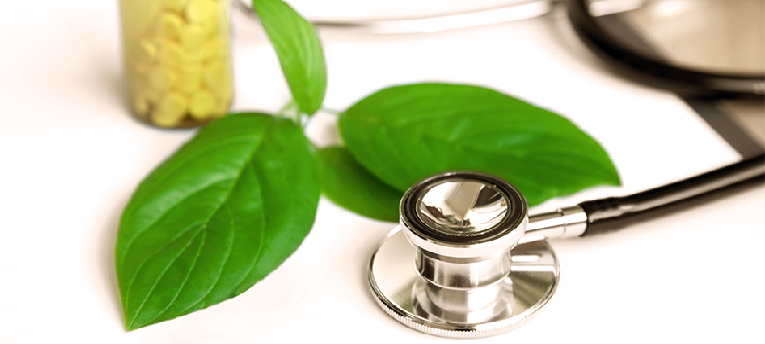
\includegraphics[width=0.47\textwidth]{naturopathyNarrow.png}
  };
\end{tikzpicture}

\hspace{-1cm}
\begin{itemize}
\item Combine 
\begin{itemize}
  \item Lit programming emphasis on documentation
  \item Code gen, but for everything
\end{itemize}
\item Codify more knowledge
\begin{itemize}
\item Physics knowledge
\item Computing knowledge
\item Document knowledge %(more than org mode)
\item Design knowledge
\item Traceability knowledge
\item Technology knowledge %(makefiles, testing frameworks, CI, etc.)
\end{itemize}

\end{itemize}

\begin{tikzpicture}[remember picture,overlay]
  \node [xshift=3.4cm,yshift=-2.0cm] at (current page.center)
  {
  
\includegraphics[width=0.47\textwidth]{generate_all_the_things.jpg}
  };
\end{tikzpicture}

\end{frame}

%%%%%%%%%%%%%%%%%%%%%%%%%%%%%%%%%%%%%%

\begin{frame}

  \frametitle{GlassBR}
  
  \begin{columns}
  \begin{column}{0.5\textwidth}
  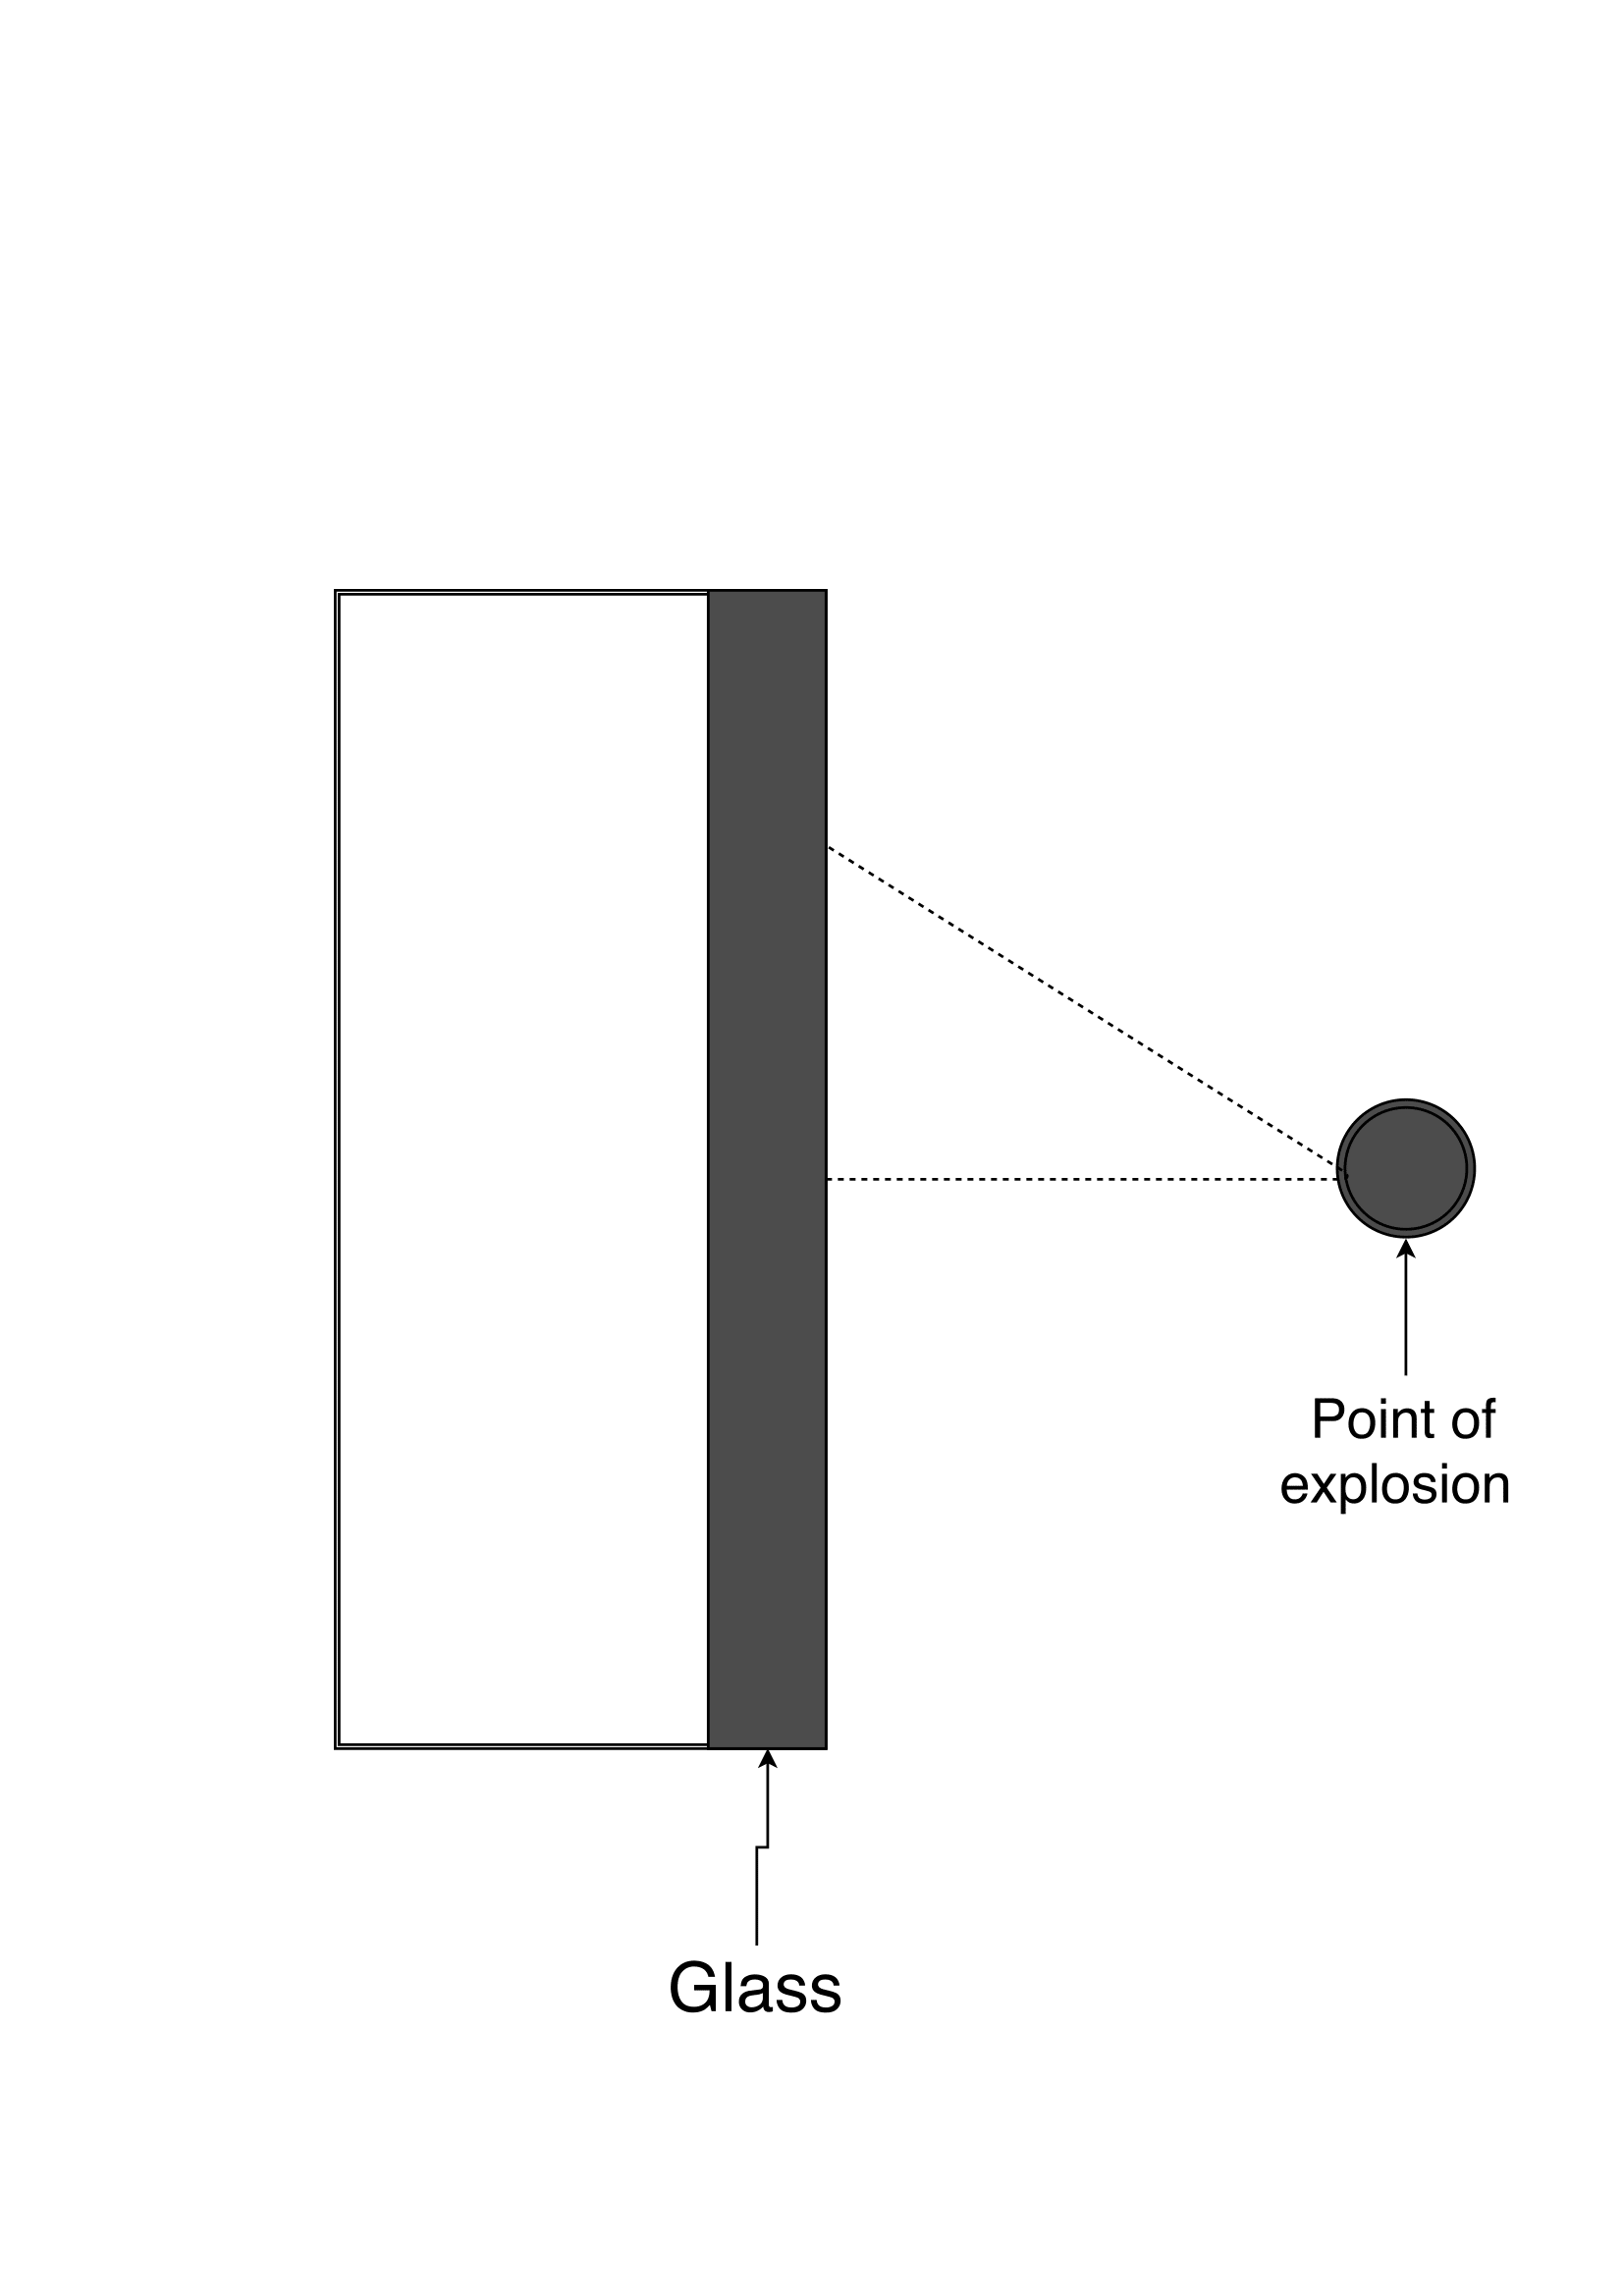
\includegraphics[width=1.0\textwidth]{physicalsystimage.png}
  \end{column}
  \begin{column}{0.5\textwidth}
  Given
  
  \begin{itemize}
  \item dimensions of plane
  \item glass type
  \item explosion characteristics
  \item tolerable breakage probability
  \end{itemize}
  
  Predict whether the glass will withstand the explosion
  
  \end{column}
  \end{columns}
  
\end{frame}
  
%%%%%%%%%%%%%%%%%%%%%%%%%%%%%%%%%%%%%%
\hoffset=-.4in %removing side bar for these frames  
\begin{frame}[plain]
  
  %\frametitle{Input Knowledge}
  
  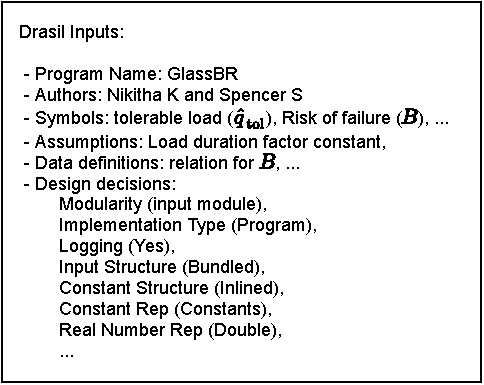
\includegraphics[width=0.95\textwidth]{DrasilInputs.pdf}
  
\end{frame}
\hoffset=0in %restore  
%%%%%%%%%%%%%%%%%%%%%%%%%%%%%%%%%%%%%%
\hoffset=-.4in %removing side bar for these frames  
\begin{frame}[plain]
  
  %\frametitle{Input Knowledge}
  
  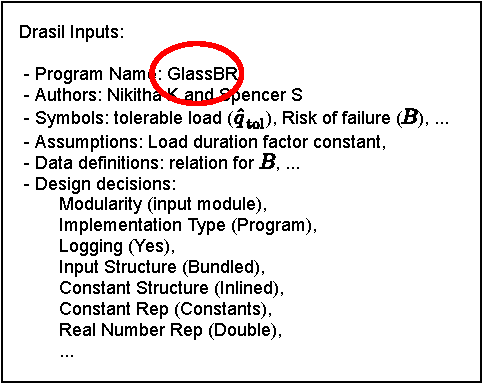
\includegraphics[width=0.95\textwidth]{InputsCircleGlassBR.pdf}
  
\end{frame}
\hoffset=0in %restore  
%%%%%%%%%%%%%%%%%%%%%%%%%%%%%%%%%%%%%%
\hoffset=-.4in %removing side bar for these frames  
\begin{frame}[plain]
  
  %\frametitle{Input Knowledge}
  
  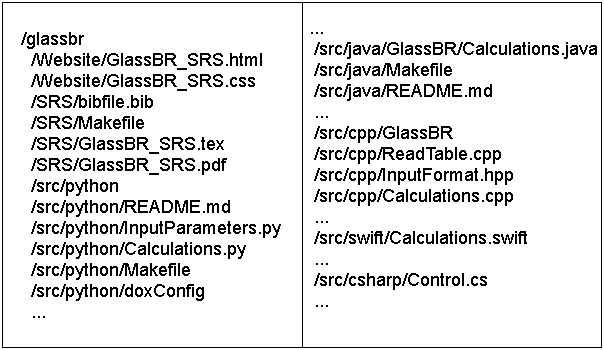
\includegraphics[width=1.05\textwidth]{FoldersFiles.pdf}
  
\end{frame}
\hoffset=0in %restore  
%%%%%%%%%%%%%%%%%%%%%%%%%%%%%%%%%%%%%%
\hoffset=-.4in %removing side bar for these frames  
\begin{frame}[plain]
  
  %\frametitle{Input Knowledge}
  
  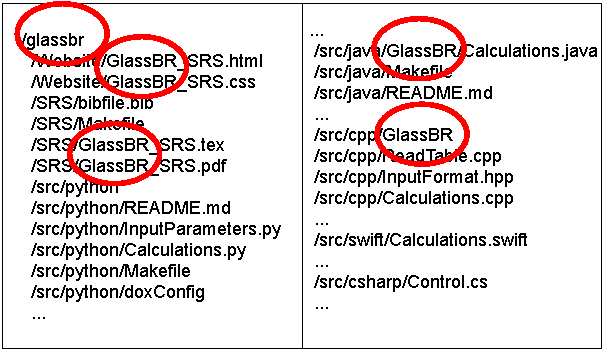
\includegraphics[width=1.05\textwidth]{FoldersFilesCircleGlassBR.pdf}
  
\end{frame}
\hoffset=0in %restore  
%%%%%%%%%%%%%%%%%%%%%%%%%%%%%%%%%%%%%%
\hoffset=-.4in %removing side bar for these frames  
\begin{frame}[plain]
  
  %\frametitle{Input Knowledge}
  
  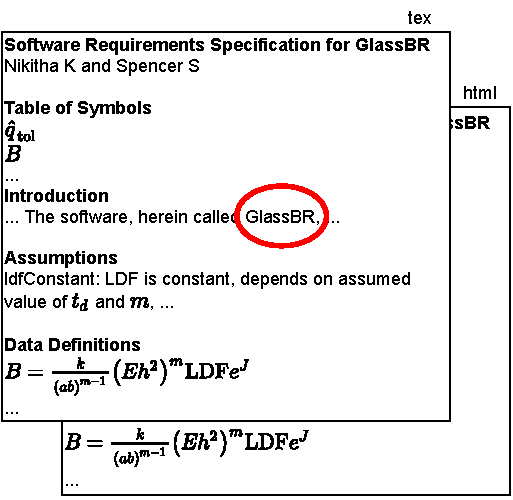
\includegraphics[width=1.05\textwidth]{SRSCircleGlassBR.pdf}
  
\end{frame}
\hoffset=0in %restore  
%%%%%%%%%%%%%%%%%%%%%%%%%%%%%%%%%%%%%%
\hoffset=-.4in %removing side bar for these frames  
\begin{frame}[plain]
  
  %\frametitle{Input Knowledge}
  
  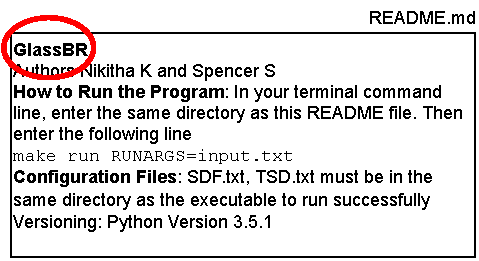
\includegraphics[width=1.05\textwidth]{READMECircleGlassBR.pdf}
  
\end{frame}
\hoffset=0in %restore  
%%%%%%%%%%%%%%%%%%%%%%%%%%%%%%%%%%%%%%
\hoffset=-.4in %removing side bar for these frames  
\begin{frame}[plain]
  
  %\frametitle{Input Knowledge}
  
  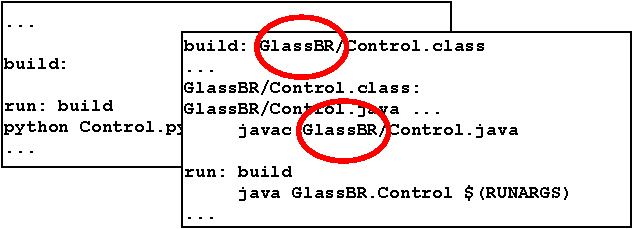
\includegraphics[width=1.05\textwidth]{MakefileCircleGlassBR.pdf}
  
\end{frame}
\hoffset=0in %restore  
%%%%%%%%%%%%%%%%%%%%%%%%%%%%%%%%%%%%%%
\hoffset=-.4in %removing side bar for these frames  
\begin{frame}[plain]
  
  %\frametitle{Input Knowledge}
  
  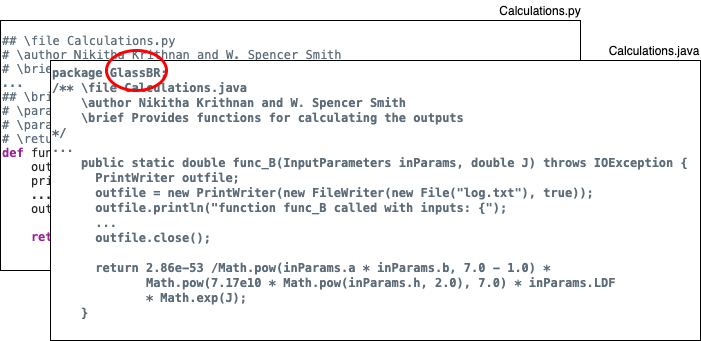
\includegraphics[width=1.05\textwidth]{CodeCircleGlassBR.png}
  
\end{frame}
\hoffset=0in %restore  
%%%%%%%%%%%%%%%%%%%%%%%%%%%%%%%%%%%%%%
\hoffset=-.4in %removing side bar for these frames  
\begin{frame}[plain]
  
  \frametitle{$J_{\mbox{tol}}$ in SRS.pdf}
  \begin{center}
  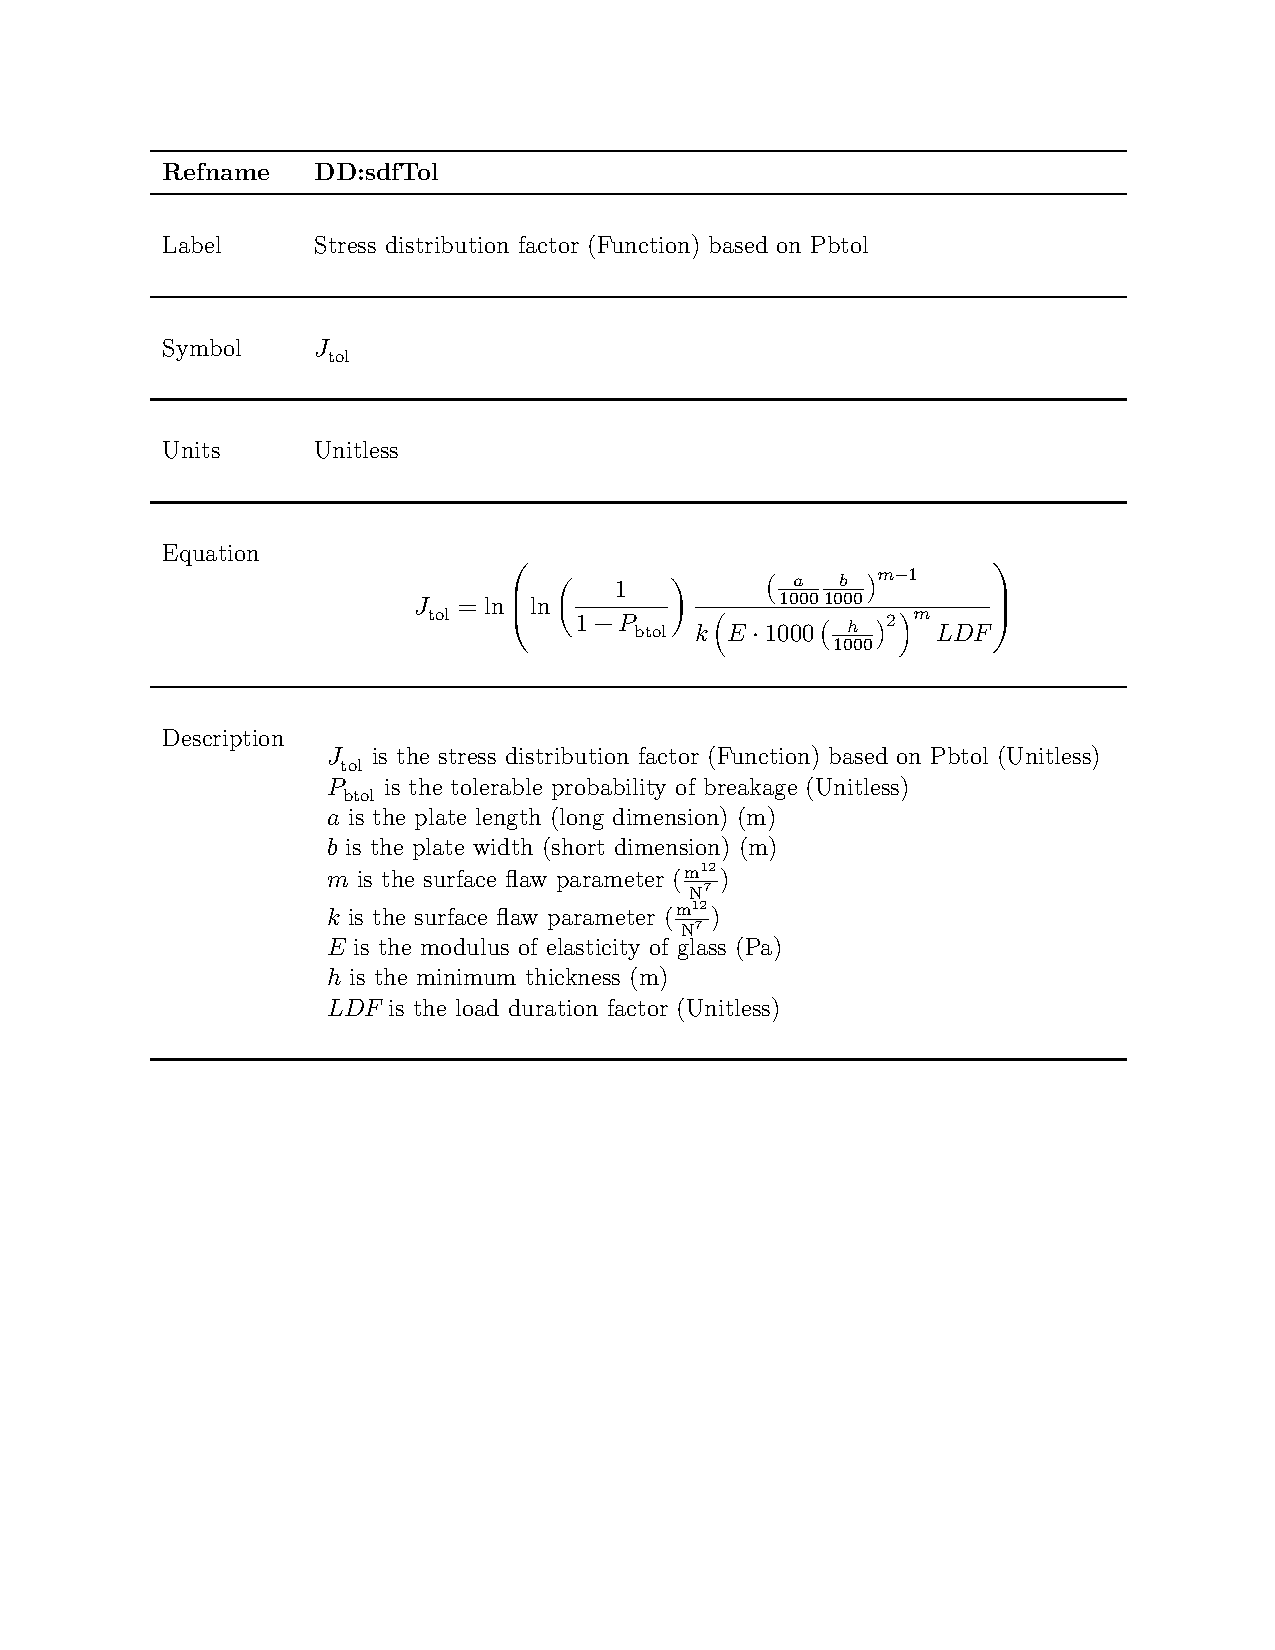
\includegraphics[width=0.9\textwidth]{Jtol_pdf.pdf}
  \end{center}
\end{frame}
\hoffset=0in %restore  
%%%%%%%%%%%%%%%%%%%%%%%%%%%%%%%%%%%%%
\hoffset=-.4in %removing side bar for these frames  
\begin{frame}[plain, fragile]
  
  \frametitle{$J_{\mbox{tol}}$ in SRS.tex}
  ~\\
  \begin{lstlisting}
  ...
  Label & Stress distribution factor (Function) based on Pbtol
          
  \\ \midrule \\
  Symbol & ${J_{\text{tol}}}$
           
  \\ \midrule \\
  Units & Unitless
          
  \\ \midrule \\
  Equation & \begin{displaymath}
             {J_{\text{tol}}}=\ln\left(\ln\left(\frac{1}{1-{P_{\text{b}\text{tol}}}}\right) \frac{\left(\frac{a}{1000} \frac{b}{1000}\right)^{m-1}}{k \left(E\cdot{}1000 \left(\frac{h}{1000}\right)^{2}\right)^{m} LDF}\right)
             \end{displaymath}
  \\ \midrule \\
  Description & ...
  \end{lstlisting}
\end{frame}
\hoffset=0in %restore    
%%%%%%%%%%%%%%%%%%%%%%%%%%%%%%%%%%%%%%
\hoffset=-.4in %removing side bar for these frames  
\begin{frame}[plain, fragile]
  
  \frametitle{$J_{\mbox{tol}}$ in SRS.html}
  
  \begin{lstlisting}
  
  ...
  <th>Equation</th>
  <td>
  \[{J_{\text{tol}}}=\ln\left(\ln\left(\frac{1}{1-{P_{\text{b}\text{tol}}}}\right) \frac{\left(\frac{a}{1000} \frac{b}{1000}\right)^{m-1}}{k \left(E\cdot{}1000 \left(\frac{h}{1000}\right)^{2}\right)^{m} LDF}\right)\]
  </td>
  ...
  \end{lstlisting}
  
\end{frame}
\hoffset=0in %restore  
%%%%%%%%%%%%%%%%%%%%%%%%%%%%%%%%%%%%%
\hoffset=-.4in %removing side bar for these frames  
\begin{frame}[plain, fragile]
  
  \frametitle{$J_{\mbox{tol}}$ in Python}
  
  \begin{lstlisting}
  ## \brief Calculates stress distribution factor (Function) based on Pbtol
  # \param inParams structure holding the input values
  # \return stress distribution factor (Function) based on Pbtol
  def func_J_tol(inParams):
      outfile = open("log.txt", "a")
      print("function func_J_tol called with inputs: {", file=outfile)
      print("  inParams = ", end="", file=outfile)
      print("Instance of InputParameters object", file=outfile)
      print("  }", file=outfile)
      outfile.close()
      
      return math.log(math.log(1.0 / (1.0 - inParams.P_btol)) * ((inParams.a / 1000.0 * (inParams.b / 1000.0)) ** (7.0 - 1.0) / (2.86e-53 * (7.17e10 * 1000.0 * (inParams.h / 1000.0) ** 2.0) ** 7.0 * inParams.LDF)))
  \end{lstlisting}
\end{frame}
\hoffset=0in %restore    
%%%%%%%%%%%%%%%%%%%%%%%%%%%%%%%%%%%%%%
\hoffset=-.4in %removing side bar for these frames  
\begin{frame}[plain, fragile]
  
  \frametitle{$J_{\mbox{tol}}$ in Java}
  
  \begin{lstlisting}
      /** \brief Calculates stress distribution factor (Function) based on Pbtol
          \param inParams structure holding the input values
          \return stress distribution factor (Function) based on Pbtol
      */
      public static double func_J_tol(InputParameters inParams) throws IOException {
          PrintWriter outfile;
          outfile = new PrintWriter(new FileWriter(new File("log.txt"), true));
          ...
          return Math.log(Math.log(1.0 / (1.0 - inParams.P_btol)) * (Math.pow(inParams.a / 1000.0 * (inParams.b / 1000.0), 7.0 - 1.0) / (2.86e-53 * Math.pow(7.17e10 * 1000.0 * Math.pow(inParams.h / 1000.0, 2.0), 7.0) * inParams.LDF)));
      }
  \end{lstlisting}
\end{frame}
\hoffset=0in %restore    
%%%%%%%%%%%%%%%%%%%%%%%%%%%%%%%%%%%%%%
\hoffset=-.4in %removing side bar for these frames  
\begin{frame}[plain, fragile]
  
  \frametitle{$J_{\mbox{tol}}$ in Drasil (Haskell)}
  
  \begin{lstlisting}
  
  tolStrDisFacEq :: Expr
  tolStrDisFacEq = ln (ln (recip_ (exactDbl 1 $- sy pbTol))
    `mulRe` (((sy plateLen $/ exactDbl 1000) `mulRe` (sy plateWidth $/ exactDbl 1000)) $^ (sy sflawParamM $- exactDbl 1) $/
      (sy sflawParamK `mulRe` ((sy modElas `mulRe` exactDbl 1000 `mulRe`
      square (sy minThick $/ exactDbl 1000)) $^ sy sflawParamM) `mulRe` sy lDurFac)))
  
  \end{lstlisting}
\end{frame}
\hoffset=0in %restore    
%%%%%%%%%%%%%%%%%%%%%%%%%%%%%%%%%%%%%%
\hoffset=-.4in %removing side bar for these frames  
\begin{frame}[plain, fragile]
  
  \frametitle{$J_{\mbox{tol}}$ without Unit Conversion}
  
  \begin{lstlisting}
  tolStrDisFacEq :: Expr
  tolStrDisFacEq = ln (ln (recip_ (exactDbl 1 $- sy pbTol))
    `mulRe` ((sy plateLen `mulRe` sy plateWidth) $^ (sy sflawParamM $- exactDbl 1) $/
      (sy sflawParamK `mulRe` ((sy modElas `mulRe`
      square (sy minThick)) $^ sy sflawParamM) `mulRe` sy lDurFac)))
  \end{lstlisting}
\end{frame}
\hoffset=0in %restore    
%%%%%%%%%%%%%%%%%%%%%%%%%%%%%%%%%%%%%%
  
\begin{frame}
  
  %\frametitle{Input Knowledge}
  
  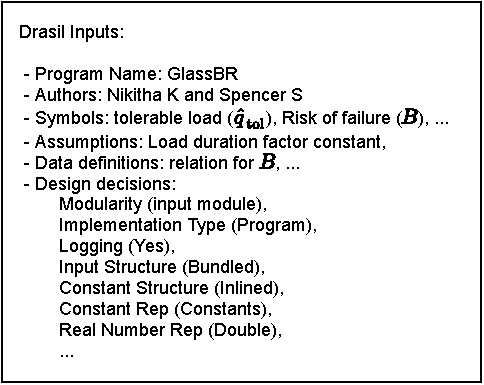
\includegraphics[width=0.95\textwidth]{DrasilInputs.pdf}
  
  \href{https://github.com/JacquesCarette/Drasil}{Drasil}
  \citep{CaretteEtAl2021-Drasil}

\end{frame}
  
%%%%%%%%%%%%%%%%%%%%%%%%%%%%%%%%%%%%%%
\hoffset=-.4in %removing side bar for these frames    
\begin{frame}[plain]

  \begin{tikzpicture}[remember picture,overlay]
    \node [xshift=0.8cm,yshift=0.0cm] at (current page.center)
    {
    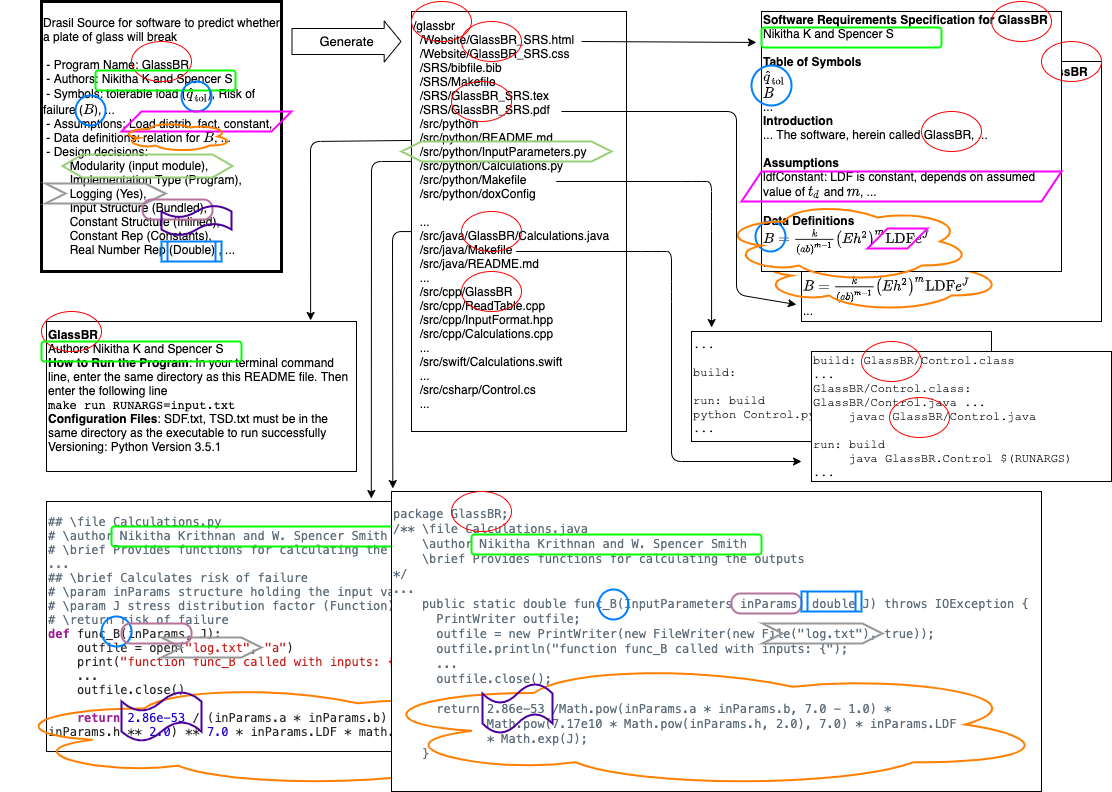
\includegraphics[width=1.2\textwidth]{DrasilSupportsChange.png}
    };
  \end{tikzpicture}
  
\end{frame}
\hoffset=0in %restore  
%%%%%%%%%%%%%%%%%%%%%%%%%%%%%%%%%%%%%%
  
\begin{frame}
  
  \frametitle{Holistic Treatment and Side Effects}
  
  \begin{itemize}
  \item Sustainable and reproducible
  \item Can generate literate documents, if desired
  \item Pain point scores:
  \begin{itemize}
      \item Lack of time: \greencheck %HELPS %-- save time by generation
      \item Lack of dev exp: \greencheck %HELPS %-- can select design decisions
      \item Lack of technology exp: \greencheck %HELPS %-- can generate technology
      \item Freq of change: \greencheck %HELPS %-- code and doc are easily updated, in sync
  \end{itemize}
  \item Treats all pain points, and no side effects, but expensive medicine!
  \end{itemize}
  
\end{frame}
  
%%%%%%%%%%%%%%%%%%%%%%%%%%%%%%%%%%%%%%
  
\section[Conclusion]{Concluding Remarks}

%%%%%%%%%%%%%%%%%%%%%%%%%%%%%%%%%%%%%%

\begin{frame}
  
  \frametitle{Concluding Remarks}
  
  \begin{itemize}
  \item Documentation \emph{does not have to be painful}
  \item Combine benefits of Literate Programming
  \begin{itemize}
    \item Emphasis on documentation, reproducibility
    \item Organize information for a human being
  \end{itemize}
  \item with benefits of Code Generation
  \begin{itemize}
    \item \emph{Capture knowledge only once}
    \item \emph{Generate all things!}
    \item \emph{Refactoring by regenerating}
  \end{itemize}
  \item \emph{Codify as much knowledge as possible}
  \item \emph{Domain experts work at domain expert level}
  \item \emph{Consistent by construction}
  \item Can address additional pain points
  \item Can absorb other treatment options, like testing, CI
  \item Requires additional research and ``clinical trials''
  \end{itemize}
  
\end{frame}
    
%%%%%%%%%%%%%%%%%%%%%%%%%%%%%%%%%%%%%%
  
\begin{frame}[allowframebreaks]
\frametitle{References}
\bibliography{Holistic}
\bibliographystyle{plainnat}
\end{frame}

%%%%%%%%%%%%%%%%%%%%%%%%%%%%%%%%%%%%%%

\begin{frame}
\frametitle{Image Credits}

\begin{itemize}
\item \href{https://www.newsmax.com/fastfeatures/holistic-medicine-websites-advice/2014/10/09/id/597217/} {Holistic Medicine: 6 Websites for Finding Natural Healing Advice}
\item \href{https://www.youngstownortho.com/spine/} {Pain \& Spine Center}
\item
\href{https://www.arksurgicalhospital.com/the-symptoms-of-a-rotator-cuff-injury-and-what-you-should-do-3/}
{The Symptoms of a Rotator Cuff Injury and What You Should Do}
\item \href{https://bookriot.com/books-with-books-on-the-cover/}{16 Books Featuring Books on the Cover}
\item \href{https://www.emrindustry.com/difference-between-naturopathic-and-holistic-medicine/} {Difference Between Naturopathic and Holistic Medicine}
\end{itemize}

\end{frame}
  
\end{document}